\documentclass[10pt,a4paper,titlepage]{article}
\usepackage[utf8]{inputenc}
\usepackage{amsmath}
\usepackage{amsfonts}
\usepackage{amssymb}
\usepackage[ngerman]{babel}
\usepackage[pdftex]{graphicx}
\usepackage[vmargin=3cm, hmargin=2cm]{geometry}
\usepackage{tabularx}

\setlength{\parindent}{0pt}
\setlength{\parskip}{2pt}

\title{Entwurfsdokument}
\author{Simon Bischof \and Jan Haag \and Adrian Herrmann \and Lin Jin \and Tobias Schlumberger \and Matthias Schnetz}

\makeindex

\begin{document}

\thispagestyle {empty}
\vspace*{4cm}
\begin{center}
\begin {huge}
Entwurfsdokument\\
\end{huge}
Simon Bischof, Jan Haag, Adrian Herrmann, Lin Jin, Tobias Schlumberger, Matthias Schnetz\\
\vspace{3cm}
\begin{huge}
Praxis der Softwareentwicklung \\
Projekt 3:\\
Automatisches Pr\"{u}fen der Korrektheit von Programmen\\
Gruppe 1\\
\vspace{2cm}

\includegraphics[height=2cm]{images/Logo.pdf}\\[0.5cm]
\end{huge}
\begin{huge}
WS 2011/2012
\end{huge}
\end{center}
\newpage
\tableofcontents
\newpage

\section{Klassendiagramme}
\subsection{"Ubersicht}
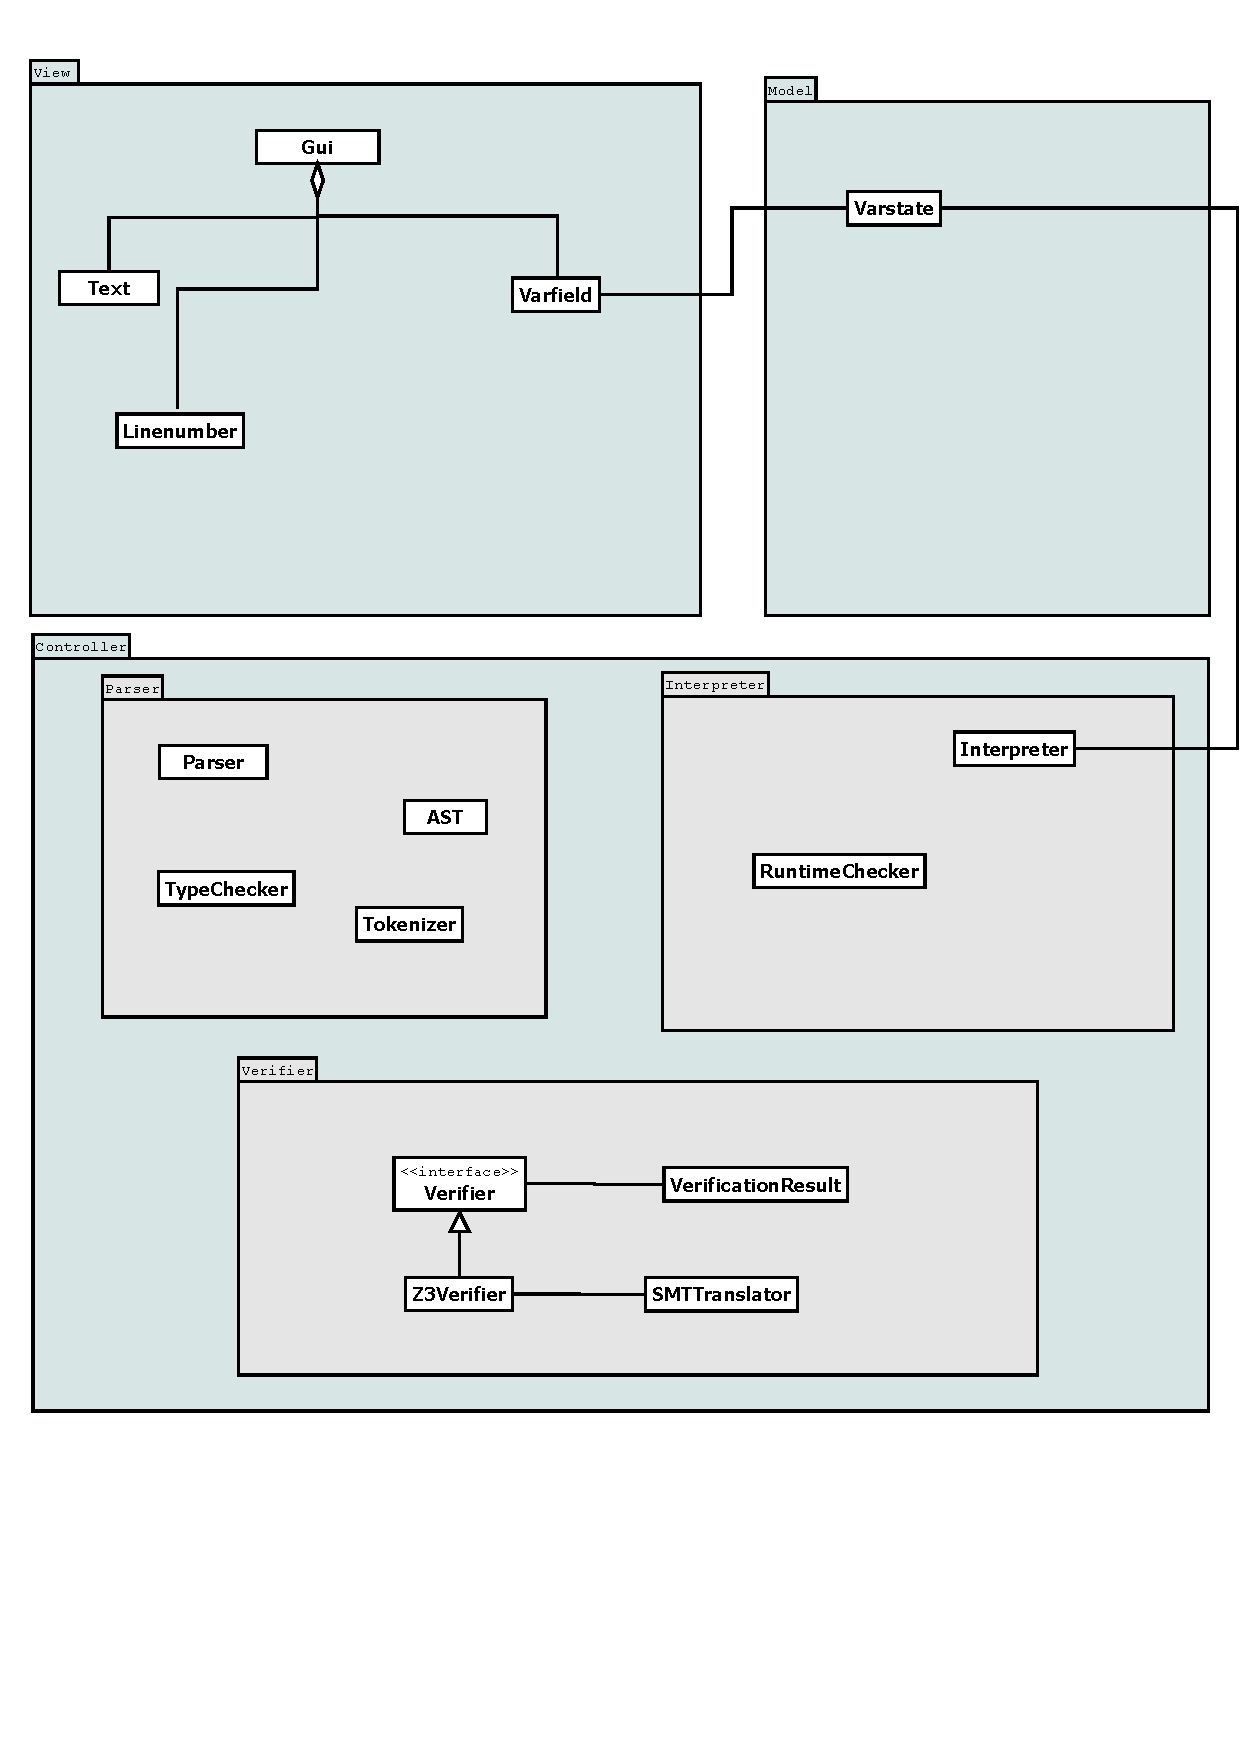
\includegraphics[scale=0.8]{images/ClassOverview.pdf}
\subsection{Feinstruktur der Komponenten}
\subsubsection{Parser}
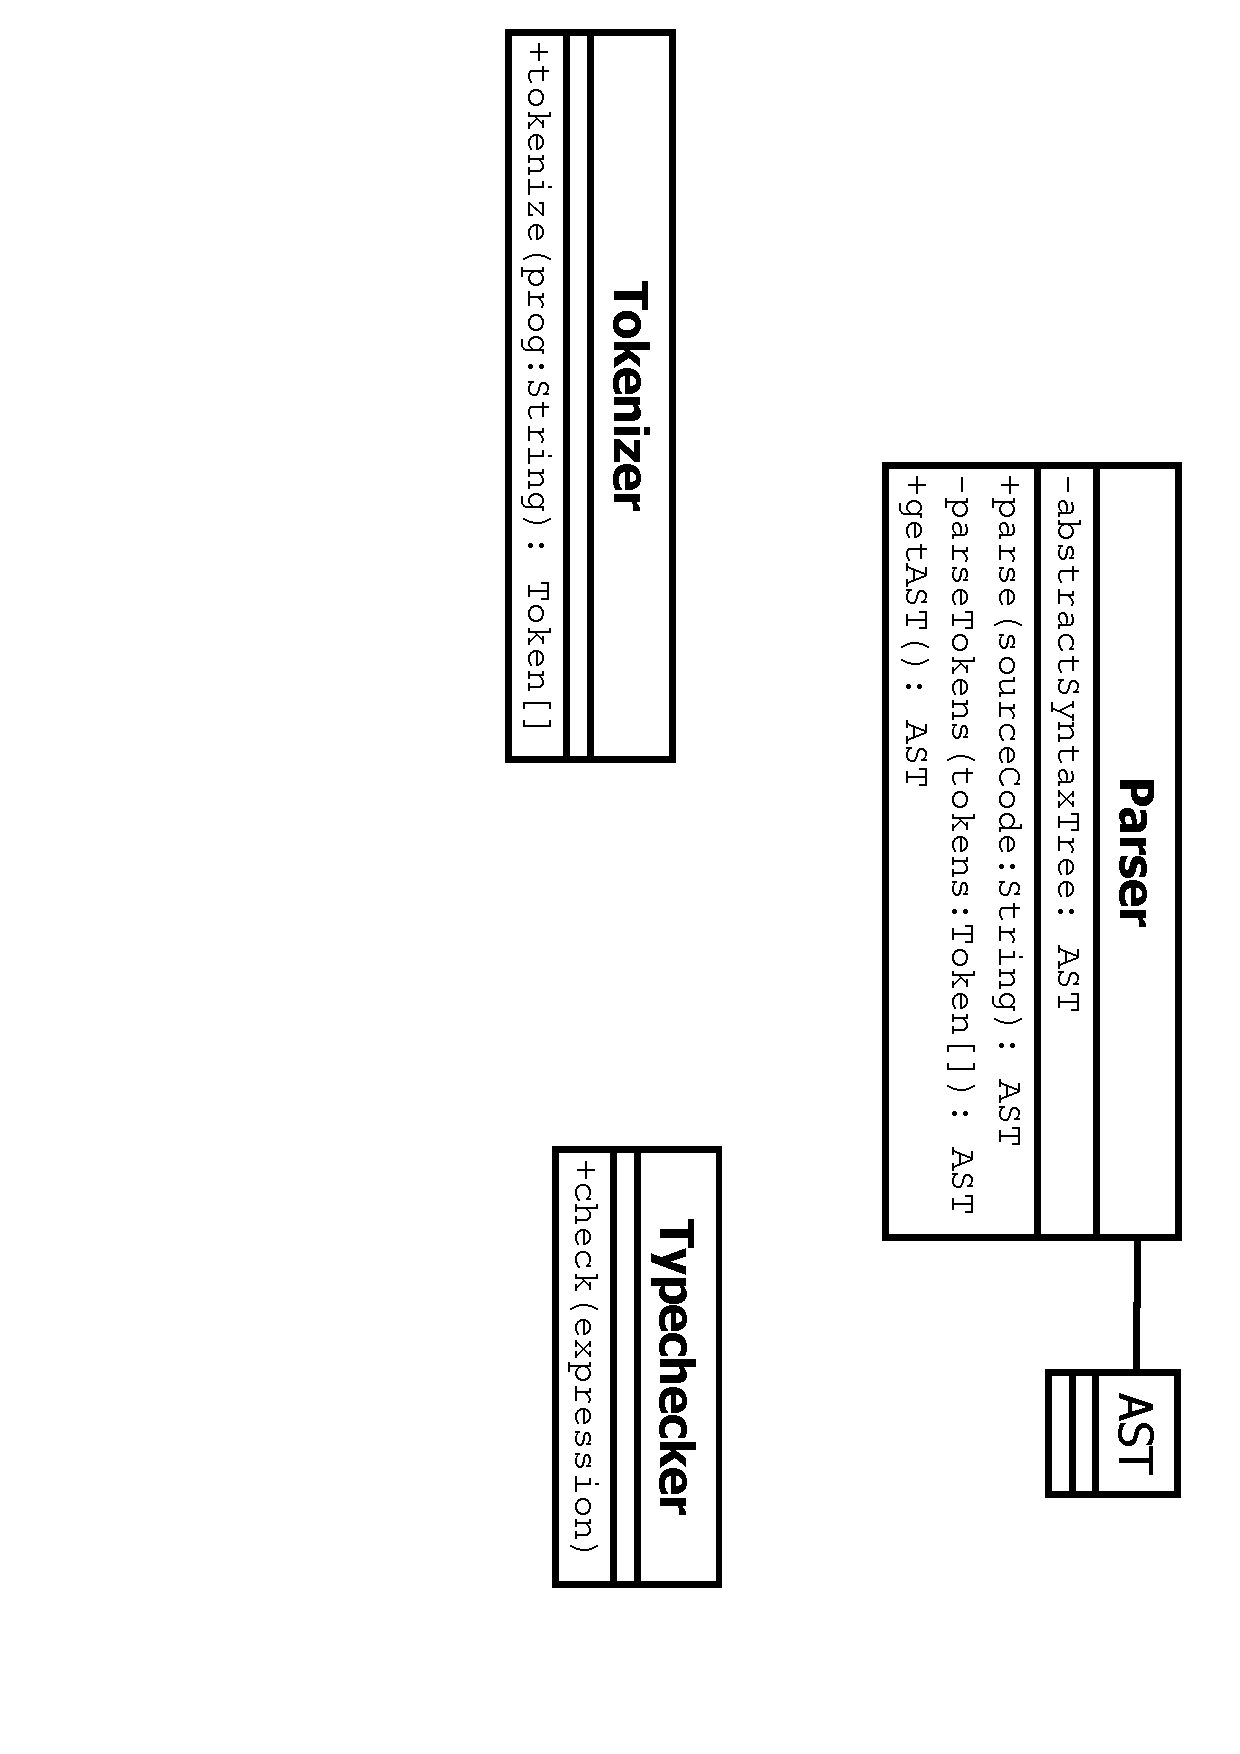
\includegraphics[angle=90, scale=0.6]{images/ClassParser.pdf}
\subsubsection{Interpreter}
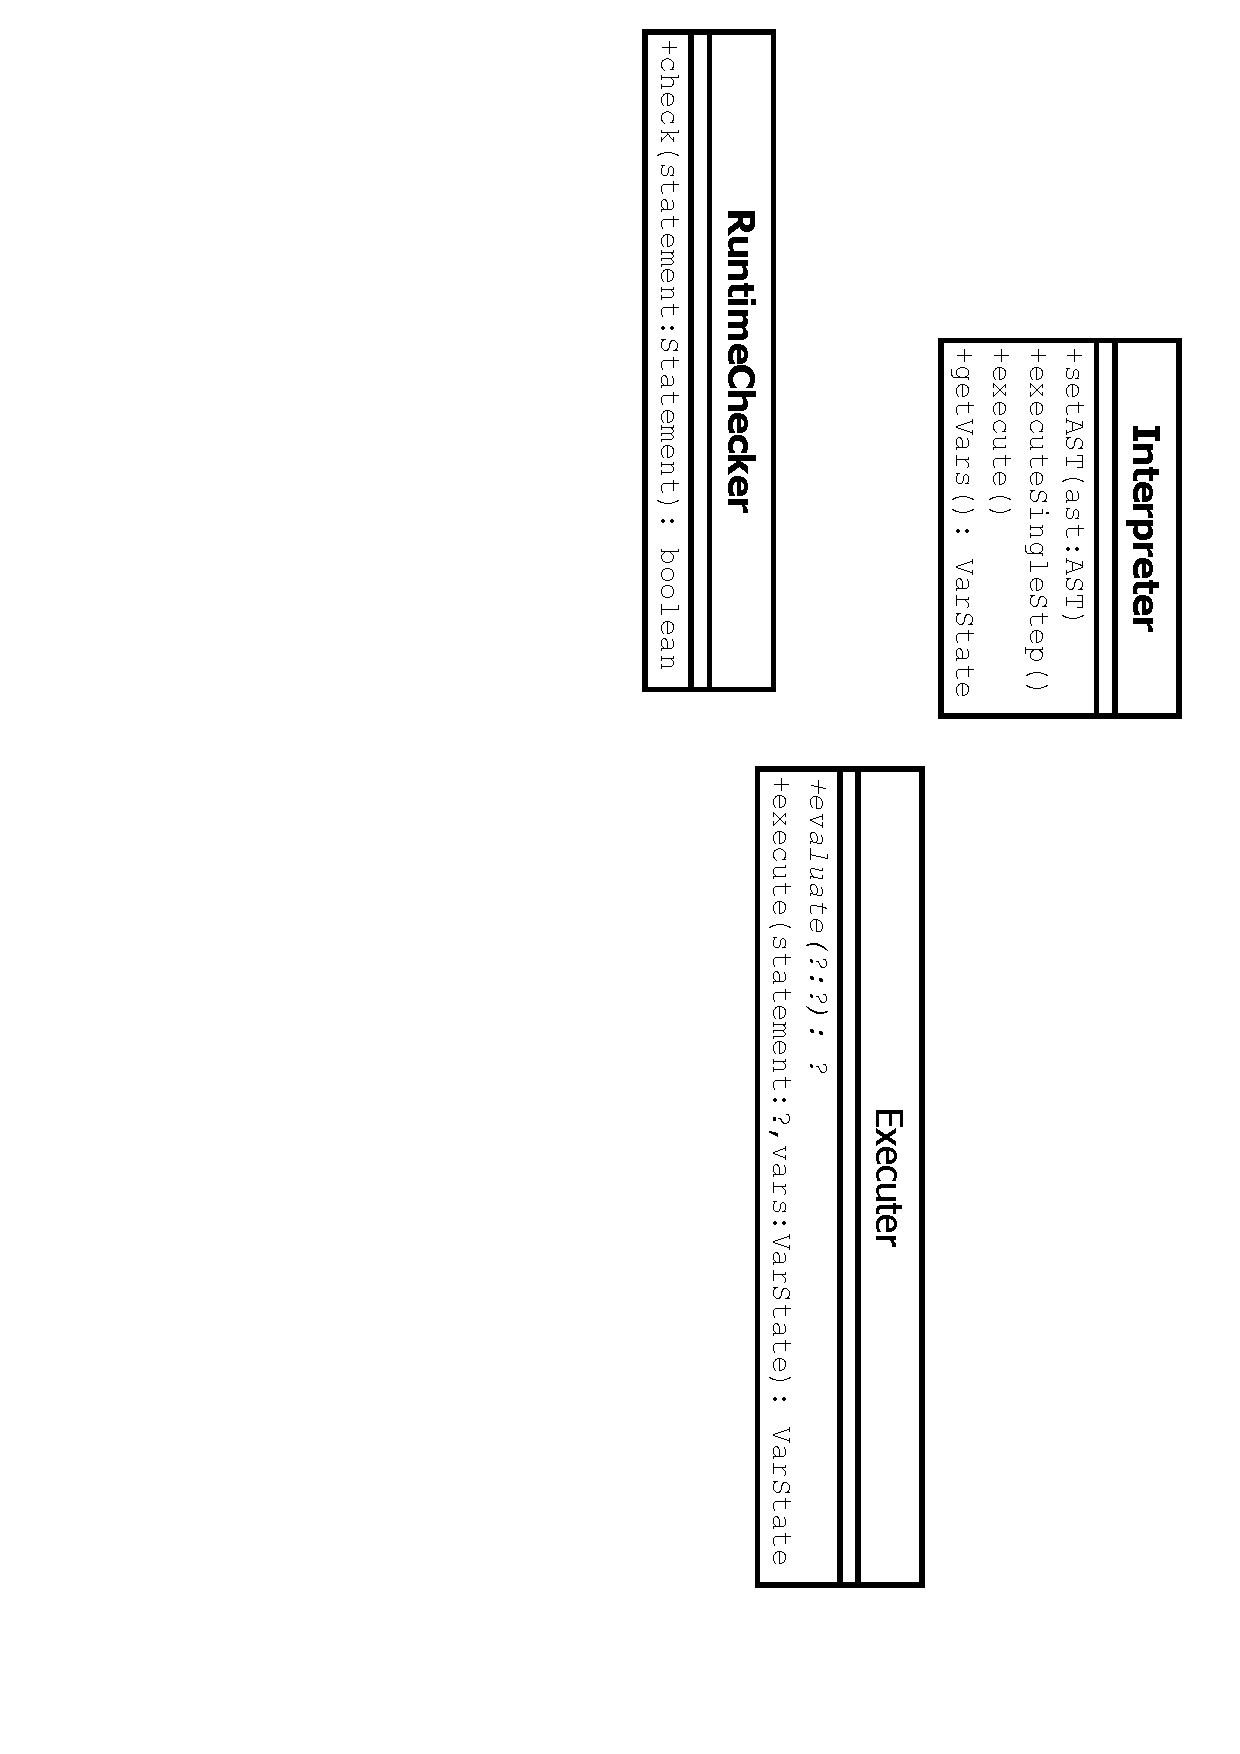
\includegraphics[angle=90, scale=0.6]{images/ClassInterpreter.pdf}
\subsubsection{Beweiser}
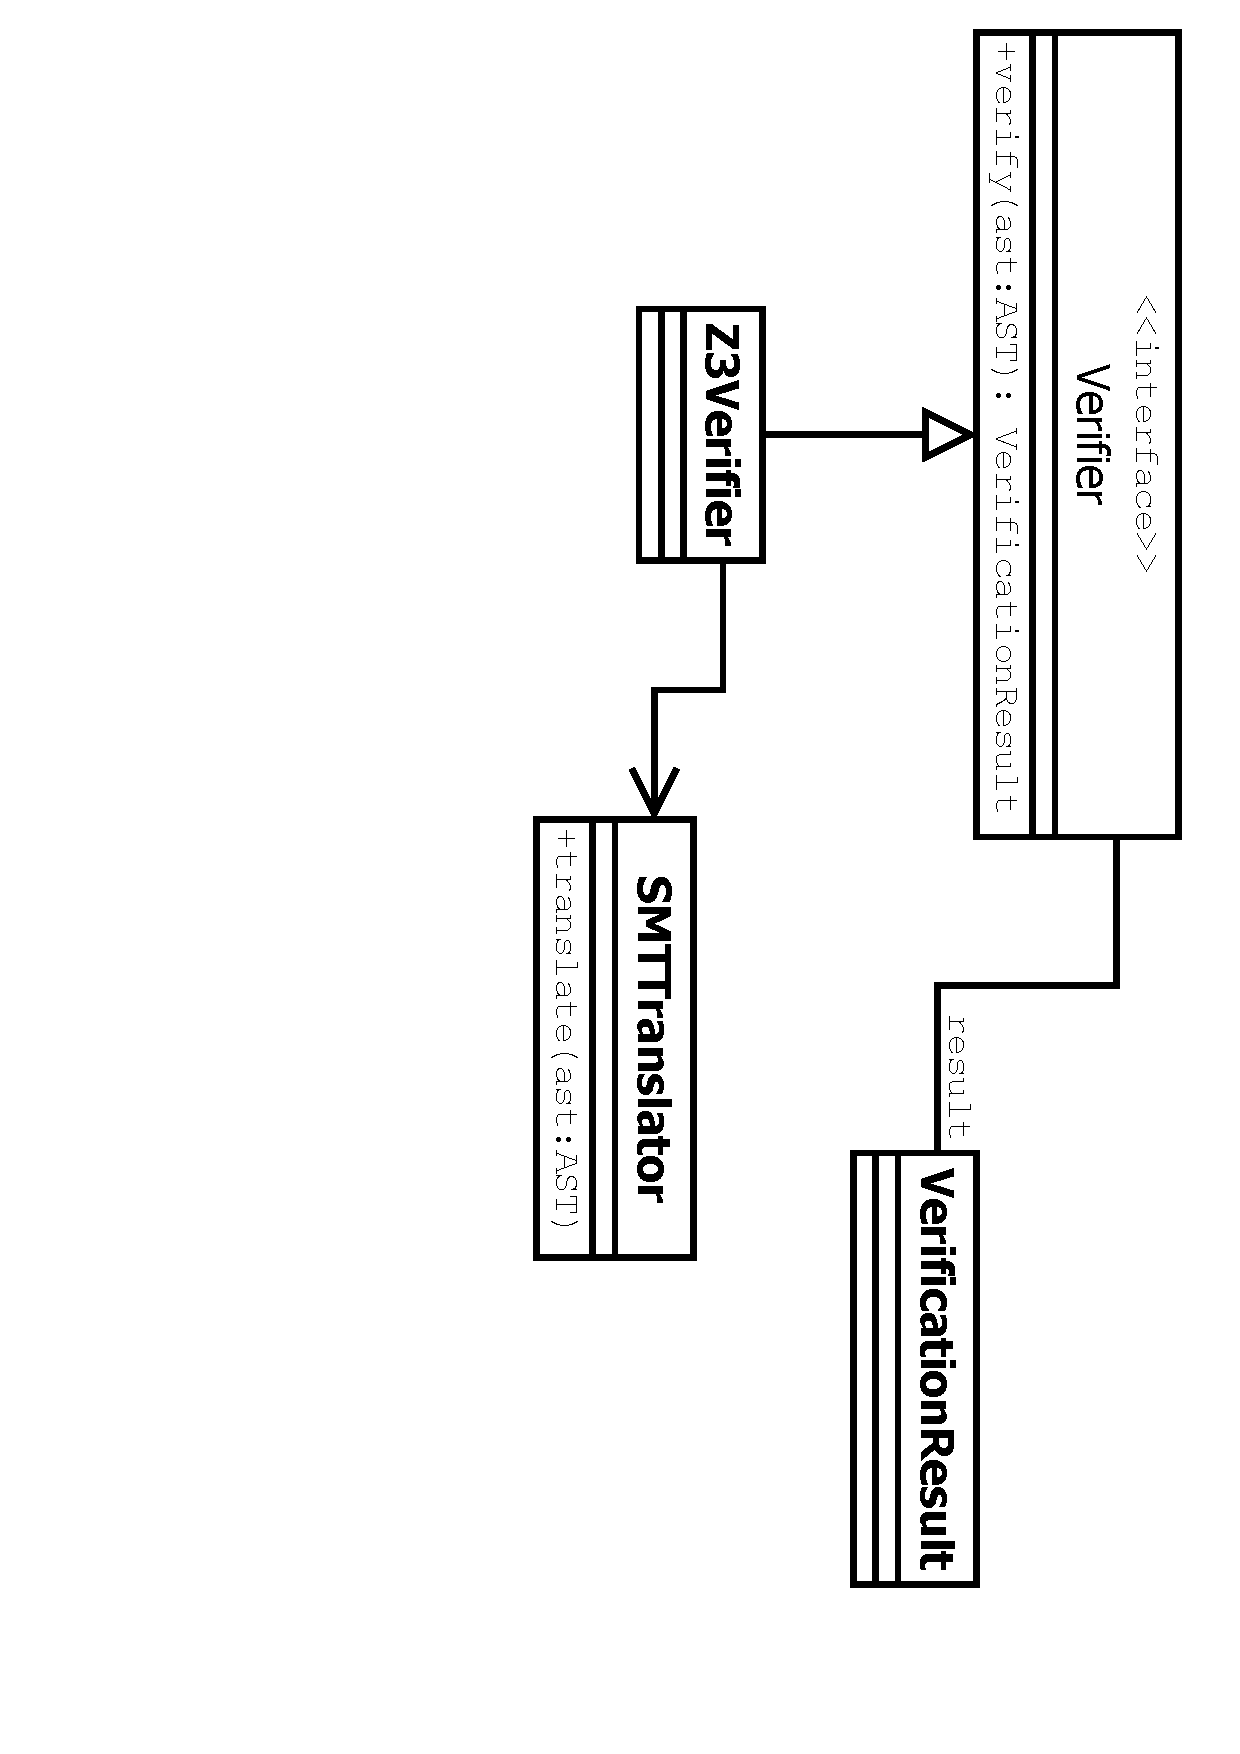
\includegraphics[angle=90, scale=0.6]{images/ClassVerifier.pdf}
\subsubsection{GUI}
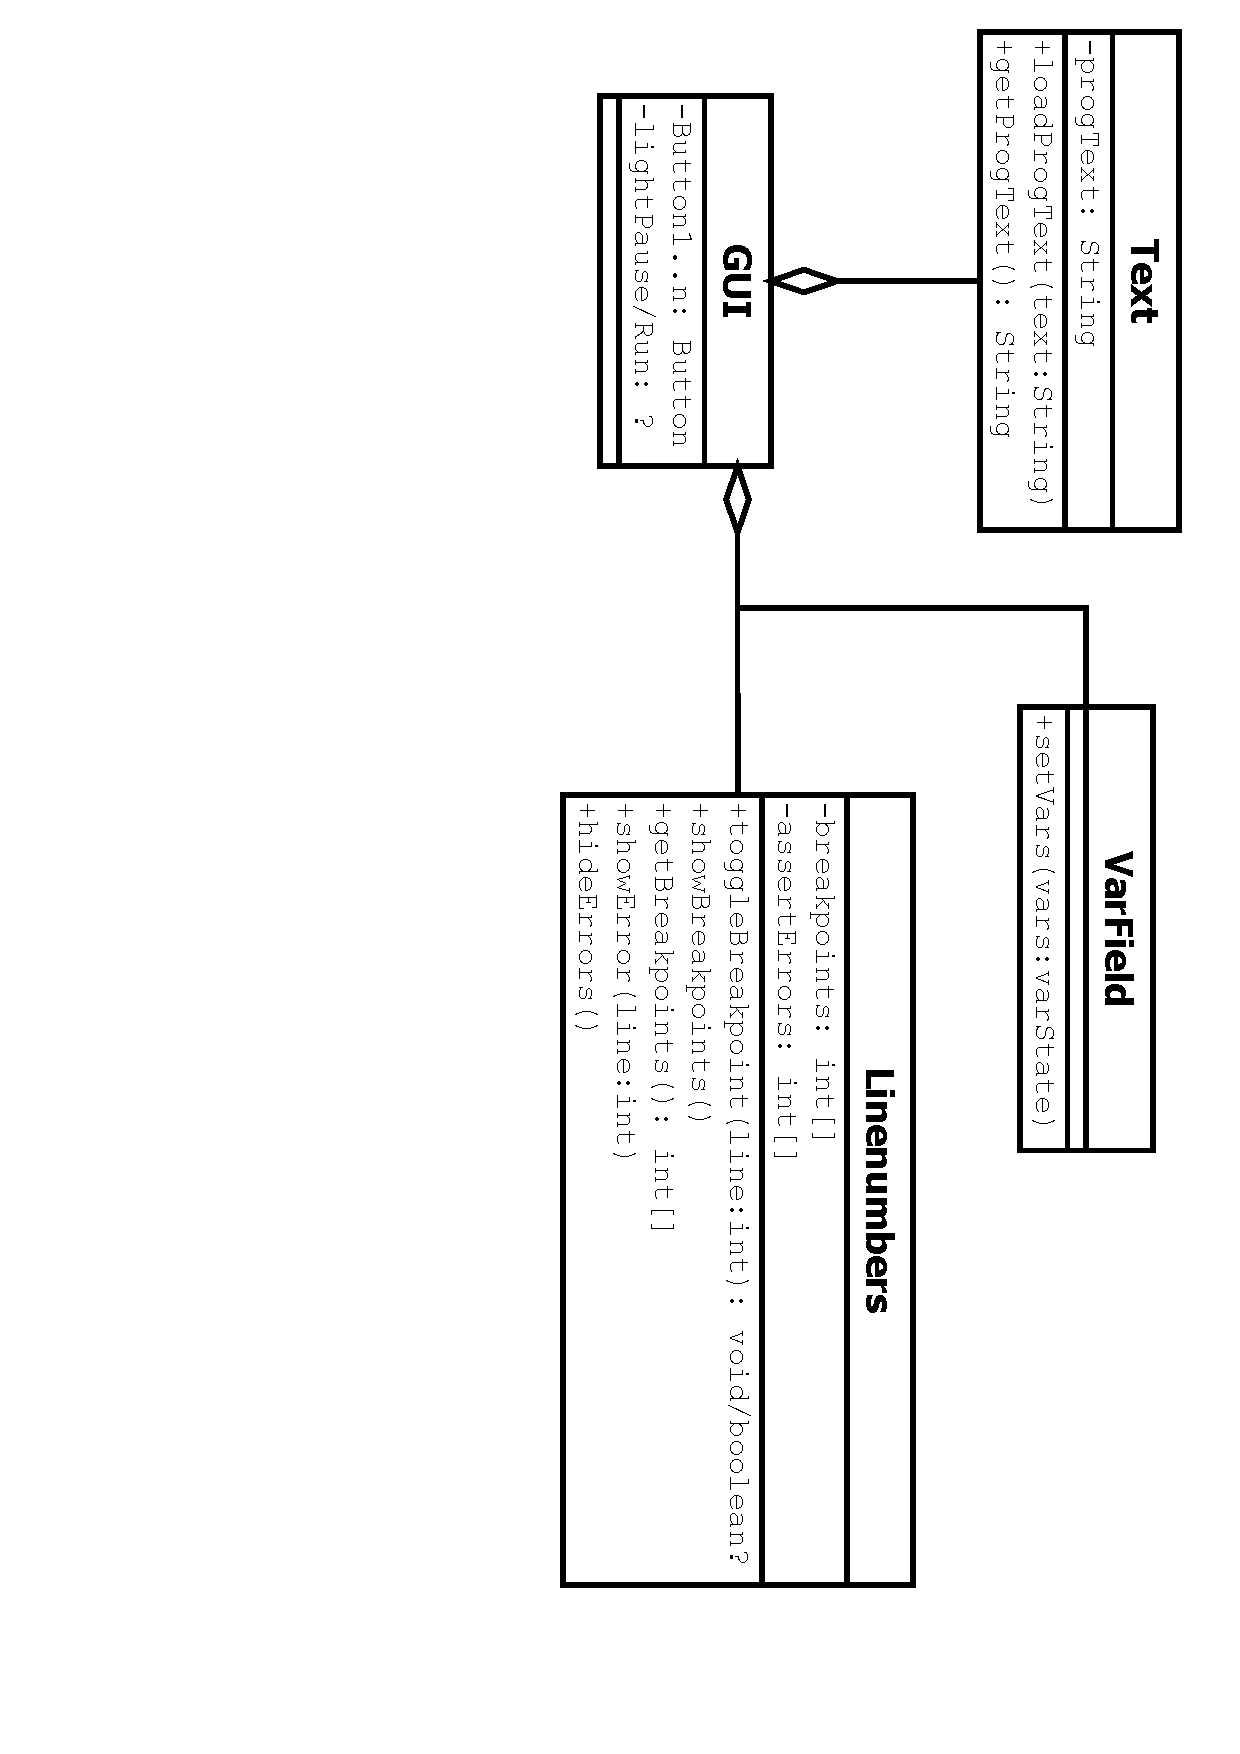
\includegraphics[angle=90, scale=0.6]{images/ClassGui.pdf}

\section{Verhaltensdiagramme}
\subsection{Aktivit"atsdiagramme}
\subsubsection{Parser/Type-Checker}
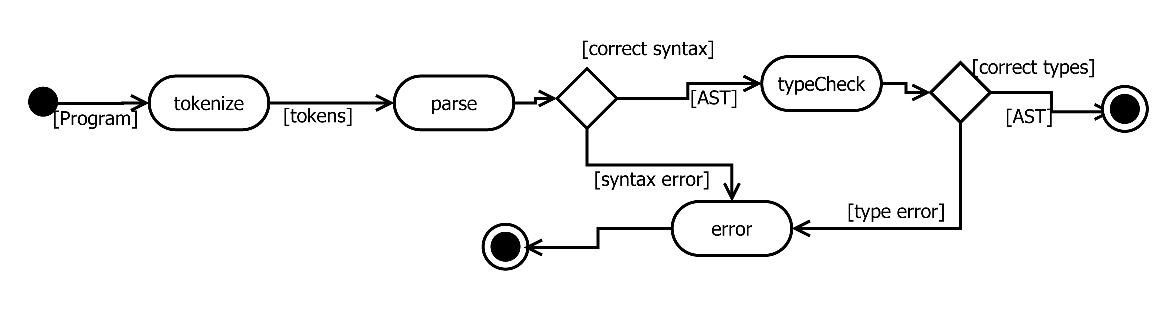
\includegraphics[angle=90, scale=0.45]{images/AktivitaetParser.pdf}\newline
Beim Aufruf des Interpreters wird das Programm in mehreren Schritten geparst.\newline
Der Programmtext wird als einzelner String dem Tokenizer übergeben, welcher den String an den wichtigen Stellen trennt und ein Array von Tokens zurückgibt. Der Parser generiert bei syntaktisch korrekte n Programmen daraus einen abstrakten Syntaxbaum (AST). Bei Syntaxfehlern bricht der Parser mit einem Fehler ab.\newline
Im Erfolgsfall überprüft der Typechecker die Korrektheit der Typen; sind die Typen korrekt, gibt dieser den vom Parser generierten AST zurück, sonst beendet er sich mit einem Fehler.
\subsection{Zustandsdiagramm}
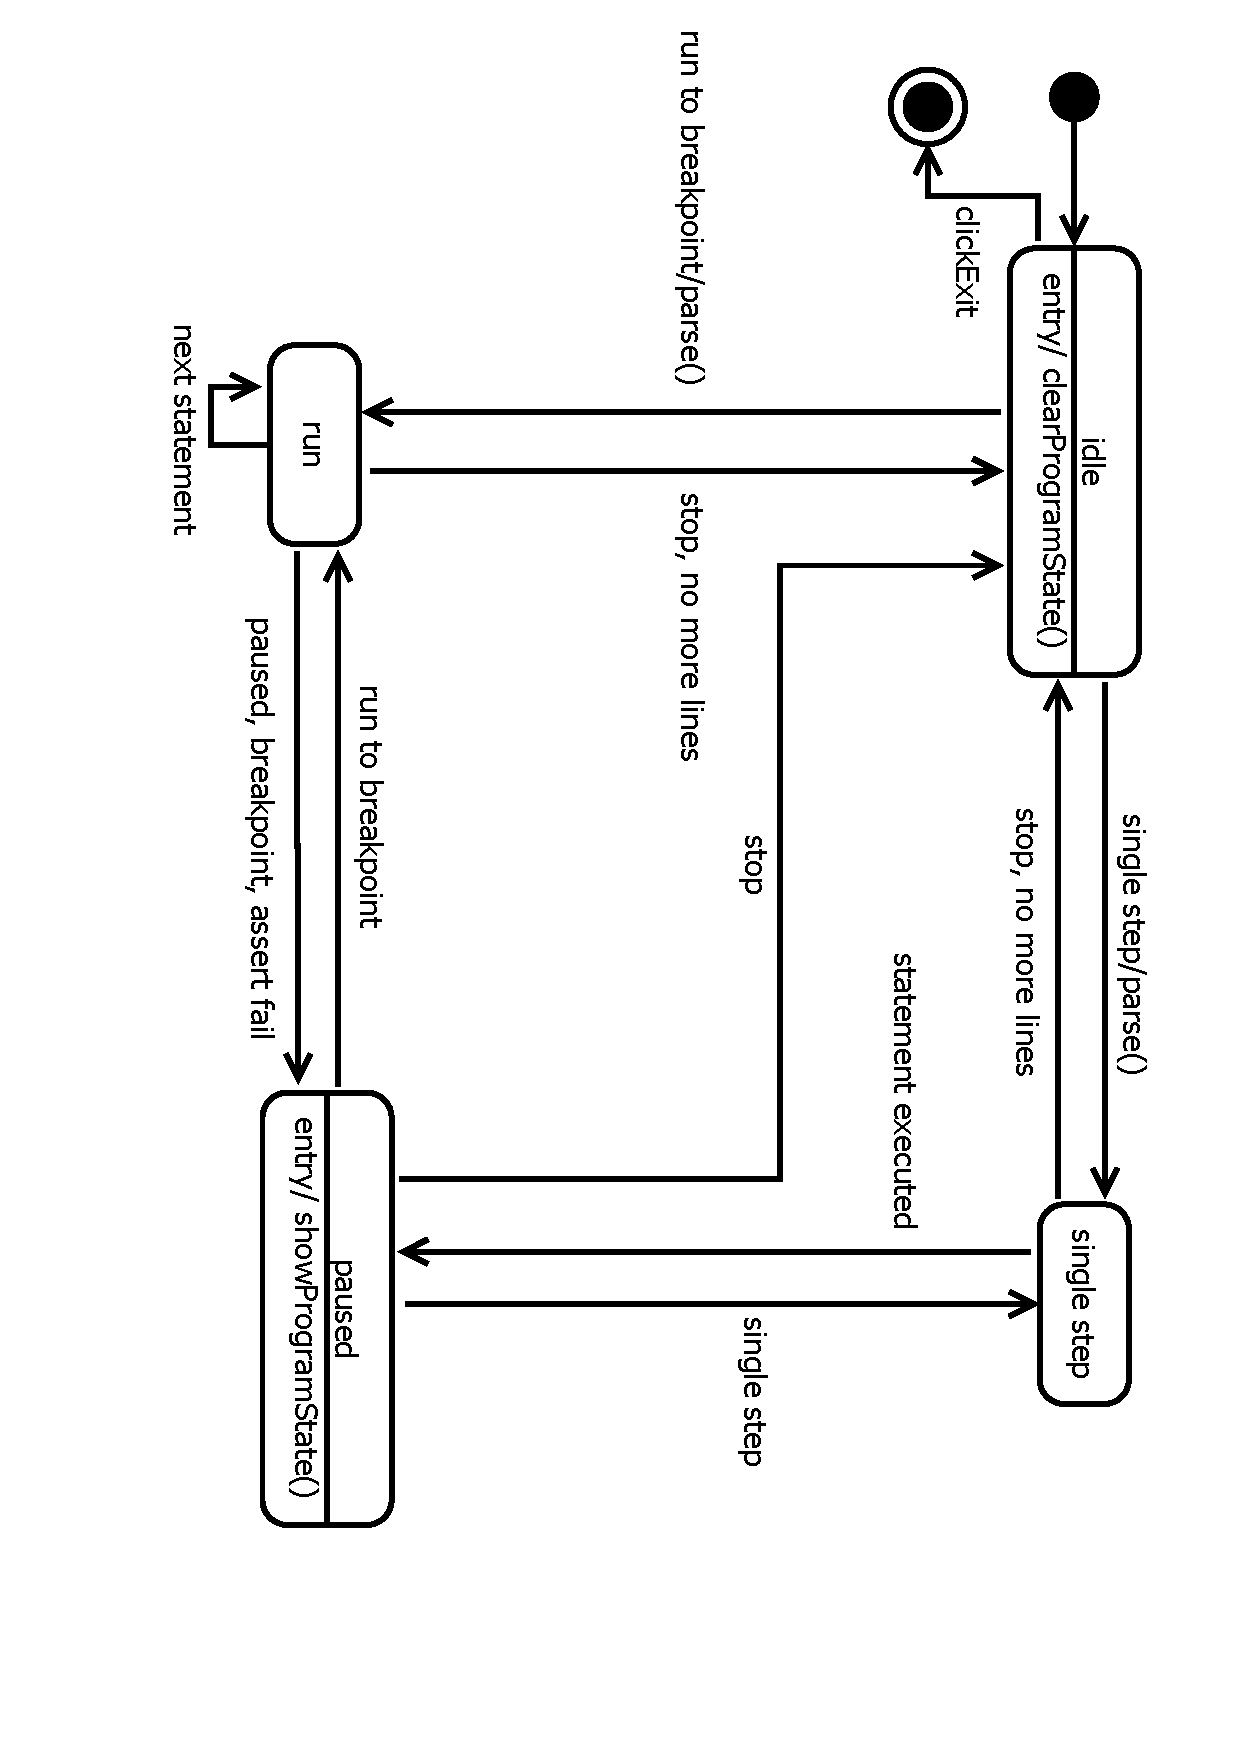
\includegraphics[angle=90, scale=0.6]{images/Zustandsdiagramm.pdf}\newline
\shorthandoff{"}
Beim Starten des Programms geht dieses in den "idle"-Zustand. Hier läuft der Interpreter nicht, und es ist kein Programmzustand gespeichert. Falls einer vorhanden ist, wird dieser beim Eintritt in den "idle"-Zustand gelöscht.\newline
Beim Auswählen von "single step" wird das Userprogramm geparst und ein Statement wird ausgeführt, nachdem der Zustand "single step" betreten worden ist. Ist kein Statement mehr vorhanden, so beendet sich der Interpreter, das Programm geht zurück in den Zustand "idle". Sonst wird nach Ausführen des Statements das Programm pausiert, der Zustand "paused" wird eingenommen. Beim Eintritt in diesen Zustand wird der Zustand des Userprogramms ausgegeben. Während der Pausierung läuft der Interpreter nicht. In diesem Zustand stehen die gleichen Möglichkeiten wie im "idle"-Zustand zu Verfügung, das Parsen bei Verlassen des Zustands entfällt aber.\newline
Wenn im "idle"-Zustand "run to breakpoint" aufgerufen wird, wird das Userprogramm geparst und das Programm geht in den Zustand "run". Das Userprogramm wird solange ausgeführt, bis es zu Ende ist (neuer Zustand: "idle") oder der Interpreter pausiert, ein Breakpoint getroffen oder eine Assertion falsifiziert wird. In diesen Fällen ist der neue Zustand "paused".\newline
In jedem Zustand außer "idle" ist es zusätzlich möglich, das Userprogramm abzubrechen, wobei der Interpreter beendet wird und alle vorhandenen Variablen-Informationen gelöscht werden. Das Programm geht danach in den Zustand "idle".\newline
In jedem Zustand kann das Programm durck einen Klick auf den Exit-Button beendet werden.
\shorthandon{"}
\newpage

\section{Syntax der While-Sprache}
\subsection{"Ubersicht der Schl"usselw"orter und Sonderzeichen}
\begin{ttfamily}
\begin{tabular}{| l  l |}
\hline
\hspace*{1.5cm}boolean & $\to$ type\_specifier\hspace*{2cm}\\\hline
\hspace*{1.5cm}else & $\to$ if\_statement\hspace*{2cm}\\\hline
\hspace*{1.5cm}false & $\to$ logical\_literal\\\hline
\hspace*{1.5cm}if & $\to$ if\_statement\\\hline
\hspace*{1.5cm}int & $\to$ type\_specifier\\\hline
\hspace*{1.5cm}return & $\to$ statement\\\hline
\hspace*{1.5cm}true & $\to$ logical\_literal\\\hline
\hspace*{1.5cm}while & $\to$ while\_statement\\\hline
\hspace*{1.5cm}0..9 & $\to$ integer\_literal\\\hline
\hspace*{1.5cm}a..z,A..Z,\_\hspace*{1cm} & $\to$ identifier\\\hline
\hspace*{1.5cm}\& & $\to$ mul\_expression\\\hline
\hspace*{1.5cm}| & $\to$ add\_expression\\\hline
\hspace*{1.5cm}! & $\to$ unary\_expression\\\hline
\hspace*{1.5cm}!= & $\to$ expression\\\hline
\hspace*{1.5cm}== & $\to$ expression\\\hline
\hspace*{1.5cm}< & $\to$ rel\_expression\\\hline
\hspace*{1.5cm}<= & $\to$ rel\_expression\\\hline
\hspace*{1.5cm}> & $\to$ rel\_expression\\\hline
\hspace*{1.5cm}>= & $\to$ rel\_expression\\\hline
\hspace*{1.5cm}+ & $\to$ add\_expression\\
 & $\to$ unary\_expression \\\hline
\hspace*{1.5cm}- & $\to$ add\_expression\\
 & $\to$ unary\_expression \\\hline
\hspace*{1.5cm}* & $\to$ mul\_expression\\\hline
\hspace*{1.5cm}/ & $\to$ mul\_expression\\\hline
\hspace*{1.5cm}\% & $\to$ mul\_expression\\\hline
\hspace*{1.5cm}, & $\to$ arglist \\
 & $\to$ parameter\_list \\
 & $\to$ variable\_declaration \\
 & $\to$ variable\_initializer\\\hline
\hspace*{1.5cm}; & $\to$ statement \\\hline
\hspace*{1.5cm}= & $\to$ variable\_declarator\\
 & $\to$ statement \\\hline
\hspace*{1.5cm}( & $\to$ bracket\_expression \\
 & $\to$ if\_statement \\
 & $\to$ while\_statement\\
 & $\to$ methode\_call \\
 & $\to$ methode\_declaration \hspace*{5cm}\\\hline
\hspace*{1.5cm}) & $\to$ bracket\_expression \\
 & $\to$ if\_statement \\
 & $\to$ while\_statement\\
 & $\to$ methode\_call \\
 & $\to$ methode\_declaration \\\hline
\hspace*{1.5cm}[ & $\to$ array\_access \\
 & $\to$ type \\\hline
\hspace*{1.5cm}] & $\to$ array\_access \\
 & $\to$ type \\\hline
\hspace*{1.5cm}\{ & $\to$ statement\_block \\
 & $\to$ variable\_initializer\\\hline
\hspace*{1.5cm}\} & $\to$ statement\_block \\
 & $\to$ variable\_initializer\\\hline
\hspace*{1.5cm}\# & $\to$ comment\\\hline
\end{tabular}
\end{ttfamily}

\subsection{Startsymbol}
\texttt{compilation\_unit}
\subsection{Produktionsregeln}
\begin{ttfamily}
\shorthandoff{"}
add\_expression ::= mul\_expression  \{ ( "|" $\mid$ "+" $\mid$ "-" ) mul\_expression \} \\\\
arglist ::=  expression \{ "," expression \}\\\\
array\_access ::= identifier "$[$" expression "$]$" \{ "$[$" expression "$]$" \} \\\\
bracket\_expression ::= "(" expression ")" \\
\hspace*{4.5cm}$\mid$ method\_call \\
\hspace*{4.5cm}$\mid$ array\_access \\
\hspace*{4.5cm}$\mid$ identifier \\
\hspace*{4.5cm}$\mid$ literal\_expression \\\\
comment ::= "\#" .* ( "\textbackslash n" $\mid$ "\textbackslash r" ) \\\\
compilation\_unit ::= \{ field\_declaration \}\\\\
expression ::= rel\_expression \{ ( "==" $\mid$ "!=" ) rel\_expression \}\\\\
field\_declaration ::= ( $[$ comment $]$ ( method\_declaration \\
\hspace*{7cm}$\mid$ statement ) )\\\\
identifier ::= "a..z,A..Z,\_" \{ "a..z,A..Z,\_,0..9" \}\\\\
if\_statement ::= "if" "(" expression ")" statement\_block $[$ "else" statement\_block $]$\\\\
integer\_literal ::= ( "0..9" \{ "0..9" \} )\\\\
literal\_expression ::= integer\_literal\\
\hspace*{4.5cm}$\mid$ logical\_literal \\\\
logical\_literal ::= "true" $\mid$ "false" \\\\
method\_call ::= identifier ( "(" $[$ arglist $]$ ")" )\\\\
method\_declaration ::= type identifier "(" $[$ parameter\_list $]$ ")" ( statement\_block )\\\\
mul\_expression ::= unary\_expression \{ ( "\&" $\mid$ "*" $\mid$ "/" $\mid$ "\%" ) 
unary\_expression \} \\\\
parameter ::= type identifier \\\\
parameter\_list ::= parameter \{ "," parameter \} \\\\
rel\_expression ::= add\_expression $[$ ( "<" $\mid$ "<=" $\mid$ ">" $\mid$ ">=" ) add\_expression $]$ \\\\
statement ::= variable\_declaration ";"\\
\hspace*{3cm}$\mid$ identifier "=" variable\_initializer ";"\\
\hspace*{3cm}$\mid$ ( expression ";" ) \\
\hspace*{3cm}$\mid$ ( if\_statement ) \\
\hspace*{3cm}$\mid$ ( while\_statement ) \\
\hspace*{3cm}$\mid$ ( "return" $[$ expression $]$ ";" ) \\\\
statement\_block ::= "\{" \{ statement \} "\}" \\\\
type ::= type\_specifier \{ "[" "]" \} \\\\
type\_specifier ::= "boolean" $\mid$ "int" \\\\
unary\_expression ::= $[$ ( "!" $\mid$ "+" $\mid$ "-" ) $]$ bracket\_expression \\\\
variable\_declaration ::= type identifier \{ "," identifier \} $[$ "=" variable\_initializer $]$ \\\\
variable\_initializer ::= expression \\
\hspace*{4.8cm}$\mid$ ( "\{" $[$ variable\_initializer \{ "," variable\_initializer \} $]$ "\}" ) \\\\
while\_statement ::= "while" "(" expression ")" statement\_block \\
\shorthandon{"}
\end{ttfamily}
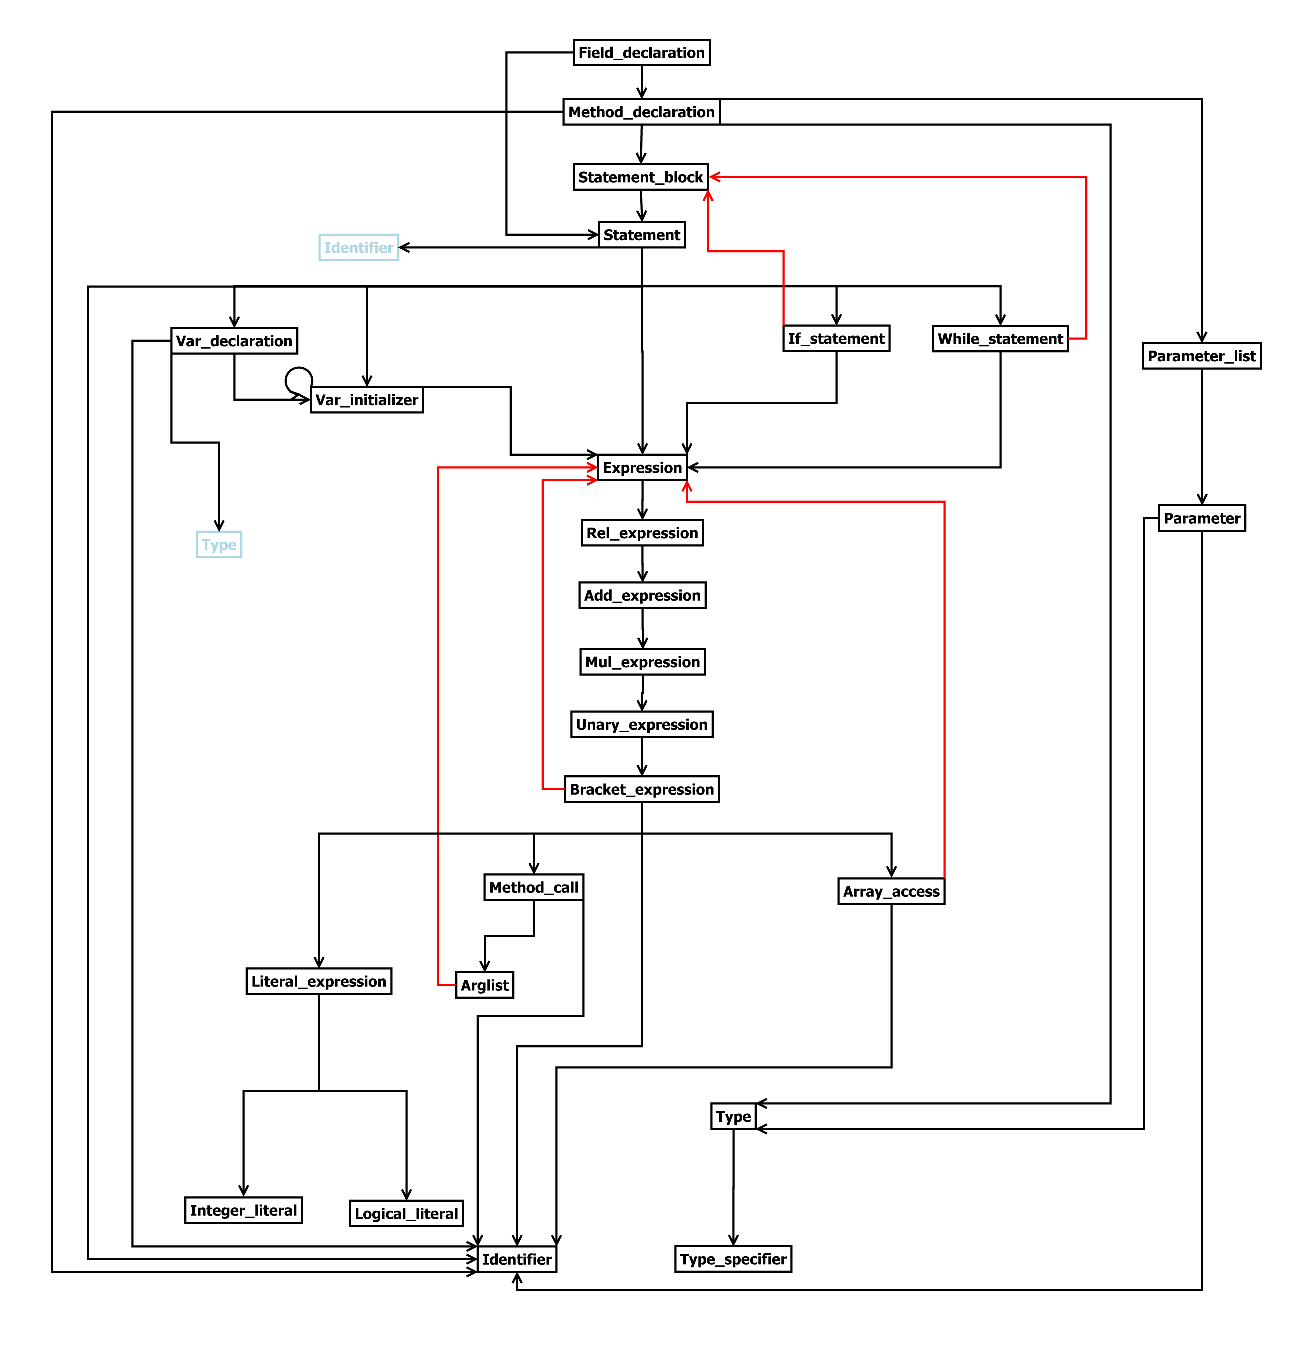
\includegraphics[scale=0.73]{images/Grammar.pdf}

\end{document}

